\documentclass[a4paper,12pt]{article}

\usepackage[utf8]{inputenc}
\usepackage[italian]{babel}
\usepackage{graphicx}
\usepackage{lipsum}
\usepackage{subcaption}
\usepackage{setspace}
\usepackage{ragged2e}

\title{\bfseries Confronto tra Alberi binari \\ \large Laboratorio di algoritmi e strutture dati}
\author{Alessandro Longo \\ Matricola 7073783}

\begin{document}

    \maketitle

    \newpage
    \tableofcontents

    \newpage


    \section{Introduzione}

    \subsection{Descrizione del problema}
    La seguente relazione ha lo scopo di confrontare i vari algoritmi di creazione di alberi binari di ricerca. In
    particolare, si prenderanno in considerazione il metodo standard e due metodi per la costruzione di alberi
    auto-bilancianti:
    \begin{itemize}
        \item la costruzione standard di alberi binari di ricerca
        \item alberi binari rosso-neri
        \item alberi AVL (Adelson-Velsky and Landis)
    \end{itemize}
    Per farlo verranno scritti dei programmi in linguaggio Python che implementino gli algoritmi di generazione di tali
    alberi e che evidenzino pro e contro di ognuno.

    \subsection{Caratteristiche del calcolatore}
    I test verranno effettuati sempre sullo stesso laptop, caratterizzato dalle seguenti specifiche:
    \begin{itemize}
        \item Processore: 12th Gen Intel Core i7-12700H CPU 2.30 GHz
        \item RAM: 16.0 GB
        \item Sistema Operativo: Windows 11 Home, versione 23H2
    \end{itemize}
    I programmi verranno scritti ed eseguiti sull’IDE PyCharm (versione 2023.2.5), mentre la relazione sarà generata
    tramite il plugin PyCharm TeXiFy IDEA, il compilatore pdfLaTeX, la distribuzione LaTeX MiKTeX e il software
    SumatraPDF.

    \par\noindent\rule{\textwidth}{0.2pt}
    \section{Analisi teorica del problema}

    \subsection{Alberi binari di ricerca}
    Gli alberi binari di ricerca sono una categoria di strutture dati che si basano su un'organizzazione gerarchica
    piramidale in cui ogni nodo ha due figli - uno destro e uno sinistro - e un genitore. La caratteristica di ogni
    nodo è che il valore del figlio sinistro è minore e quello del figlio destro è maggiore: questo semplifica molto
    operazioni come ricerca, lettura e inserimento di nuovi valori.

    La struttura dati dell'albero binario di ricerca può essere "aumentata" con statistiche d'ordine dinamiche o resa
    più efficiente se si sceglie un metodo di costruzione "height-balanced", che mantiene cioè l'altezza dell'albero
    uguale (o quasi) per tutte le foglie.
    \subsection{Implementazione delle strutture dati}

    \subsubsection{Alberi binari di ricerca}
    L'albero binario di ricerca semplice presenta dei metodi che non modificano la struttura dell'albero, come per
    esempio la ricerca di un elemento o la lettura di tutti i suoi valori, e metodi che invece alterano la posizione
    degli elementi, come l'inserimento, la cancellazione e il trapianto.

    \subsubsection{Alberi rosso-neri}
    L'albero rosso nero espande l'albero binario semplice aggiungendo l'attributo del colore ad ogni nodo, che può
    essere, appunto, o rosso o nero: questo servirà da strumento per mantenere l'albero bilanciato ad ogni operazione
    di modifica dello stesso.
    Le proprietà da mantenere vere ad ogni operazione sono:
    \begin{enumerate}
        \item Ogni nodo è rosso o nero
        \item La radice è nera
        \item Ogni foglia $T.\text{null}$ è nera
        \item Se un nodo è rosso, allora entrambi i suoi figli sono neri, quindi non esistono due rossi consecutivi in
        un cammino semplice dalla radice alla foglia
        \item Tutti i cammini da ogni nodo alle foglie contengono lo stesso numero di nodi neri
    \end{enumerate}

    \subsubsection{Alberi AVL}
    L'ultima implementazione degli alberi binari di ricerca sono gli alberi AVL - dal nome degli inventori
    Adelson-Velsky e Landis -, anch'essi alberi bilanciati, ma che invece di sfruttare l'attributo del colore usano una
    statistica d'ordine dinamica chiamata "fattore di bilanciamento", calcolata come differenza tra le "altezze" di due
    nodi. Con "altezza" si indica un'altra statistica d'ordine dinamica che indica il livello al quale si trova ogni
    nodo rispetto alla radice.

    Dopo aver inserito un nuovo valore nell'albero, a seconda del fattore di bilanciamento si possono effettuare delle
    rotazioni per bilanciarlo nuovamente e fare in modo che l'altezza delle foglie differisca di al massimo un livello.

    \subsection{Prestazioni attese}
    Per quanto riguarda le prestazioni attese, si prenderanno in considerazione il caso medio e peggiore per le due
    operazioni di ricerca e inserimento, calcolate per tutte e tre le diverse implementazioni.

    Nel caso dell'albero binario di ricerca semplice, le operazioni di inserimento e ricerca richiedono di scorrere
    l'albero fino ad una foglia, cioè al massimo un numero di elementi pari all'altezza dell'albero.
    Nel caso medio questa è proporzionale al logaritmo in base due del numero di nodi, mentre nel caso peggiore,
    che si verifica quando vengono inseriti i nodi in ordine crescente (o decrescente), l'altezza massima corrisponde
    esattamente al numero di nodi.

    \begin{figure}[h]
      \centering
      \begin{subfigure}{0.49\textwidth}
        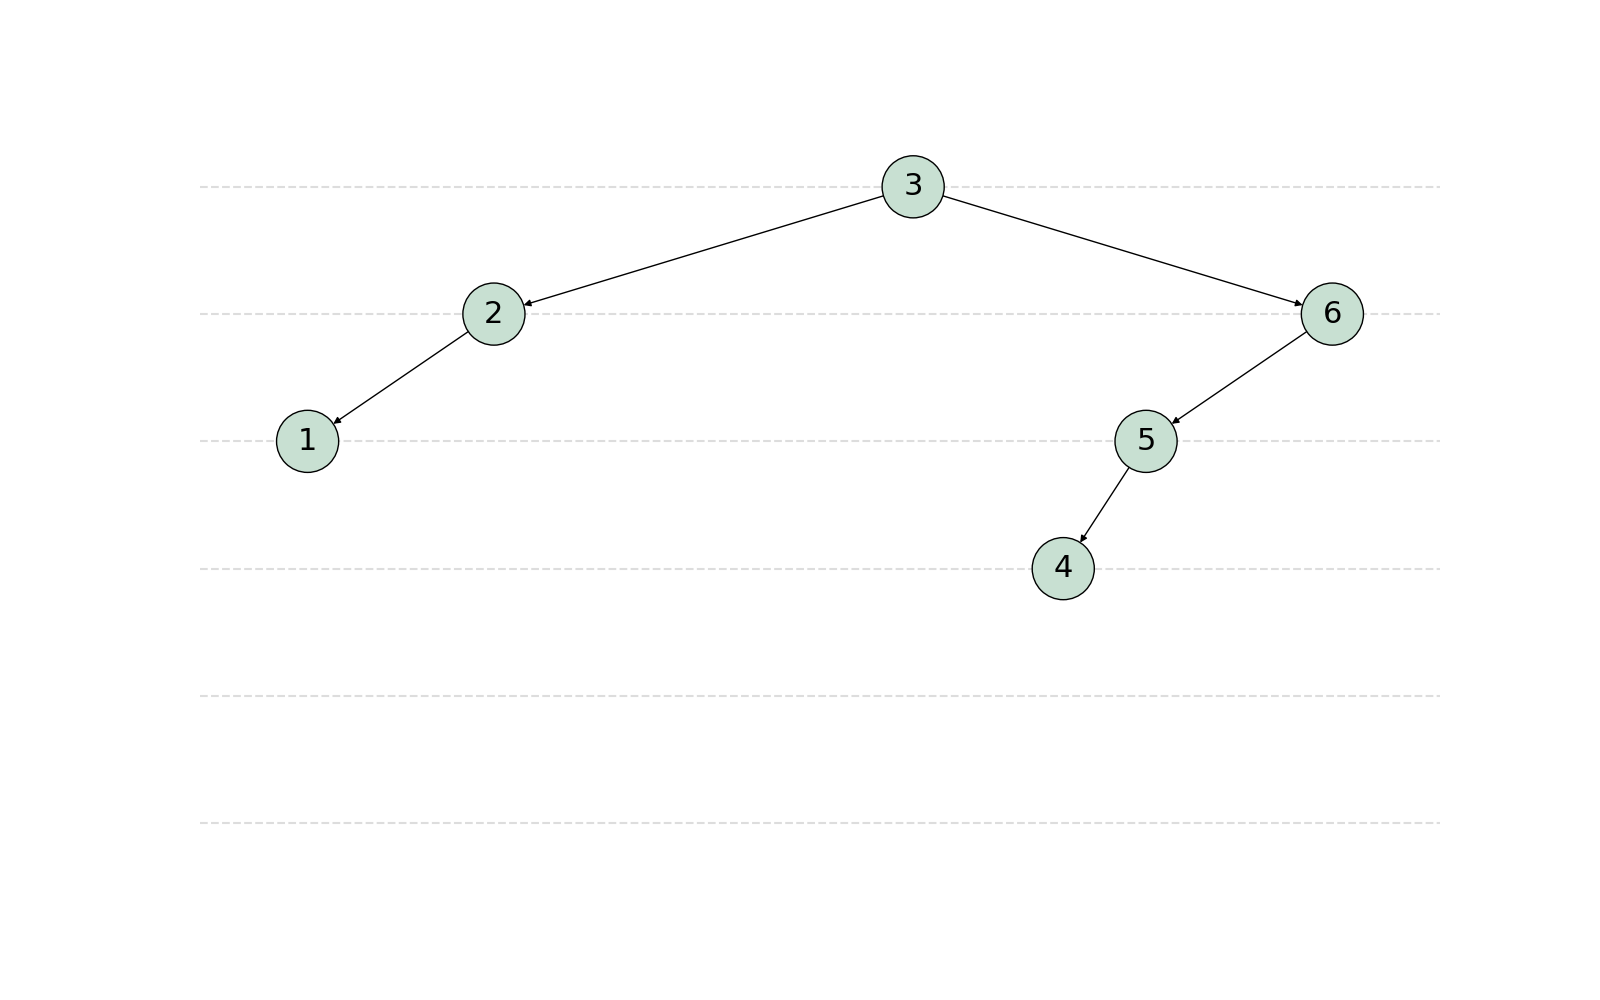
\includegraphics[width=\linewidth]{NBT insertion average case}
        \caption{Caso medio: $O(\log_2(n))$}
        \label{fig:immagine1}
      \end{subfigure}
      \hfill
      \begin{subfigure}{0.49\textwidth}
        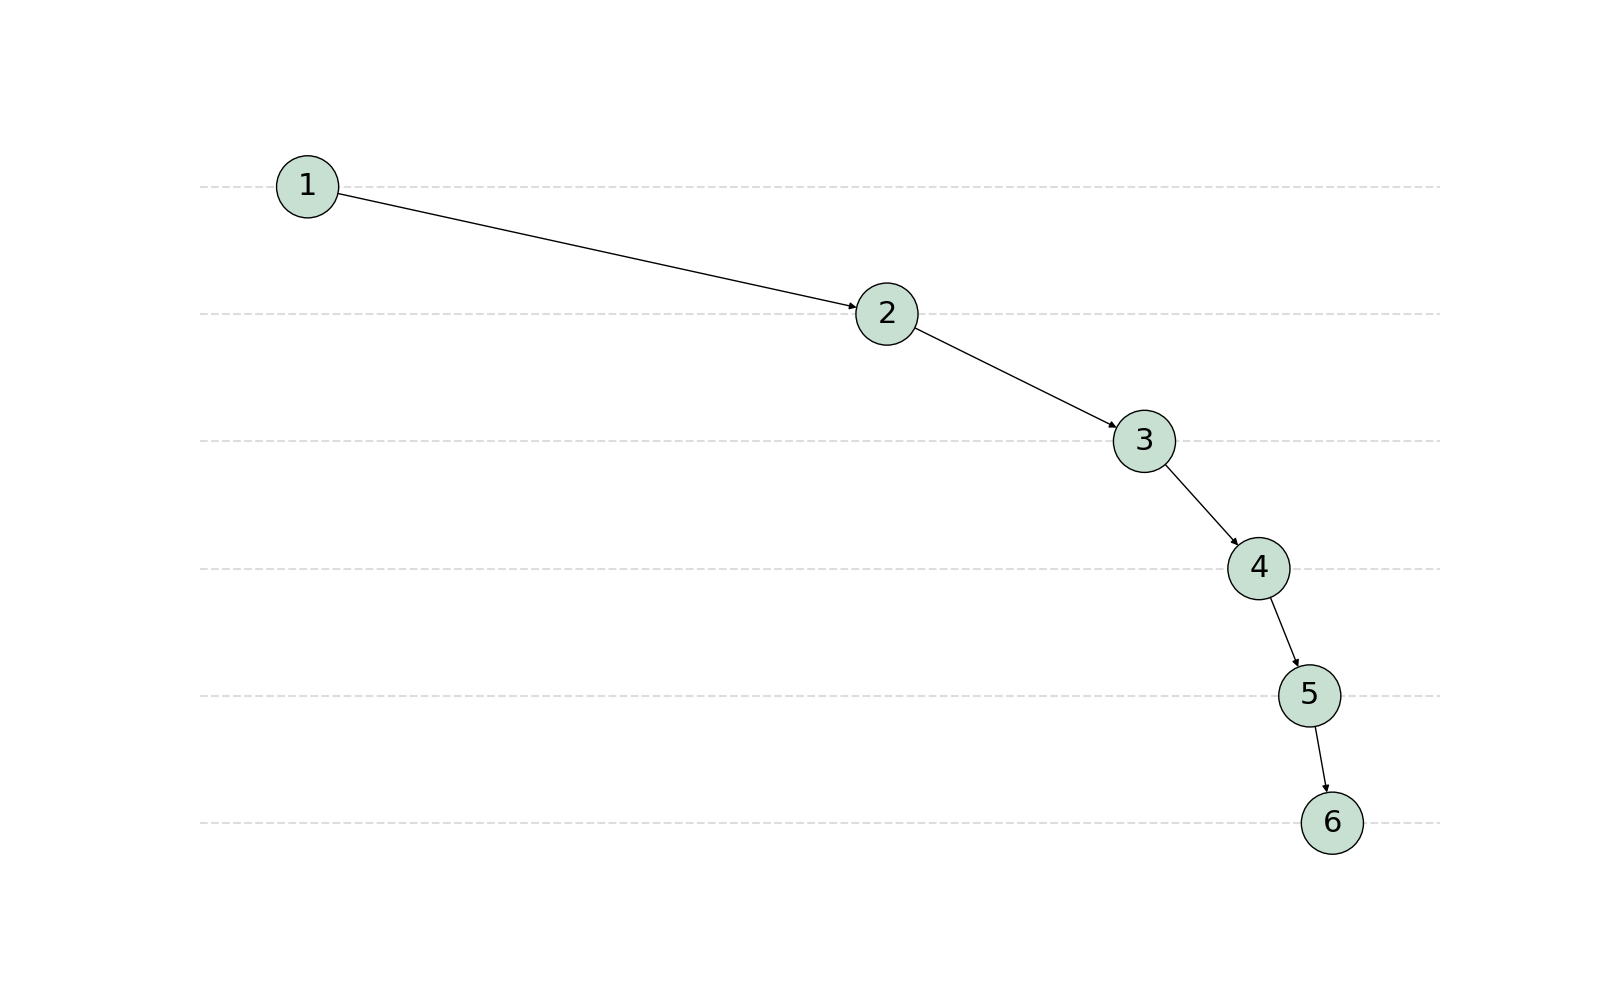
\includegraphics[width=\linewidth]{NBT insertion worst case}
        \caption{Caso peggiore: $O(n)$}
        \label{fig:immagine2}
      \end{subfigure}
      \caption{Inserimento su albero binario semplice}
      \label{fig:entrambe}
    \end{figure}

    Per l'albero rosso-nero, invece, l'operazione di ricerca ha sempre complessità logaritmica perché si tratta di una
    struttura bilanciata, quindi non c'é differenza tra caso peggiore e medio.
    L'inserimento, invece, nel un caso peggiore ha complessità logaritmica a causa delle rotazioni da effettuare nella
    fixup, mentre l'analisi ammortazzata mostra che nel caso medio ha complessità costante.

    Infine abbiamo l'albero AVL, che ha complessità logaritmica per entrambe le operazioni sia nel caso peggiore che in
    quello medio, a causa del gran numero di rotazioni previste dall'algoritmo di inserimento.

    \par\noindent\rule{\textwidth}{0.2pt}
    \section{Documentazione del codice}

    \subsection{Schema delle classi}

    \begin{figure}[h]
        \centering
        \includegraphics[width=1\textwidth]{}
        \caption{Schema UML delle classi}
        \label{fig:esempio}
    \end{figure}

    \subsection{Scelte implementative}
    Per implementare i tre diversi tipi di albero, è stata prima implementata una classe per l'albero binario di
    ricerca, che comprende un costruttore e dei metodi standard a tutti gli alberi, cioè la ricerca di un elemento,
    del precedente, successivo, minimo e massimo dell'albero, la stampa inorder e preorder.

    Successivamente sono stati implementati l'albero binario di ricerca semplice, rosso-nero e AVL estendendo la
    classe base appena descritta e ognuno implementando con metodi diversi le operazioni di modifica necessarie ad
    ognuno, come l'inserimento, il trapianto, la rotazione e la cancellazione.

    Per quanto riguarda i test, invece, è stata creata una classe TreeTester, che contiene tutti i metodi necessari
    per costruire gli alberi, eseguire i test e mostrare i risultati sotto forma di grafici.

    Inoltre, è stata implementata una classe analoga, chiamata TreePainter, che invece permette all'utente di creare
    alberi e poi disegnarli a schermo tramite le librerie matplotlib e networkx.

    \subsection{Descrizione dei metodi delle classi}
    \subsubsection{BinaryTree}
    \begin{itemize}
        \item recursive\textunderscore search(Node x, int key): prende in ingresso un nodo x e il valore da cercare (
        chiave) e ricorsivamente, scende lungo l'albero finché non la trova: se esiste un nodo con quella chiave,
        viene restituito in output; altrimenti viene restituito None
        \item iterative\textunderscore search(int key): prende in ingresso solo il valore da cercare e,
        iterativamente, parte dalla radice e scende lungo l'albero finché non trova un nodo con la chiave cercata:
        analogamente alla funczione precedente, se tale elemento esiste, viene restituito, altrimenti restituisce None
        \item minimum(Node x): percorre il sottoalbero con radice x scendendo lungo i figli sinistri fino ad una
        foglia, che poi restituisce
        \item maximum(Node x): percorre il sottoalbero con radice x scendendo lungo i figli destri fino ad una
        foglia, che poi restituisce
        \item predecessor(Node x): prende in ingresso un nodo x e restituisce il suo predecessore, cioè il nodo con
        la massima chiave minore alla sua
        \item successor(Node x): prende il ingresso un nodo x e restituisce il suo successore, cioè il nodo con la
        minima chiave maggiore alla sua
        \item get\textunderscore size(Node x): restituisce la dimesione del sottoalbero che ha come radice il nodo x
        \item get\textunderscore rank(Node x): restituisce la posizione del nodo x nella lista ordinata di elementi
        rispetto alle chiavi
        \item select\textunderscore nth(Node x, int n): tramite una ricerca ricorsiva, restituisce il nodo che
        ricopre la posizione n-esima nella lista ordinata rispetto alle chiavi
        \item update\textunderscore layers(Node x, int layer): aggiorna l'attributo
        layer del nodo x e richiama la funzione in modo ricorsivo sui due figli (se esistono) passando il layer
        incrementato di uno
        \item inorder\textunderscore walk(Node x): esegue lo scorrimento in order sull'albero, stampando i valori in
        ordine crescente
        \item preorder\textunderscore walk(Node x): esegue lo scorrimento pre order sull'albero, stampando i valori
        in notazione parentesizzata
        \item trapianto(Node u, Node v): sostituisce il sottoalbero con radice u con quello con radice v modificando
        semplicemente i puntatori dei nodi
        \item clear(): resetta l'albero assegnando alla radice il valore None
    \end{itemize}

    \subsubsection{NormalBinaryTree}
    \begin{itemize}
        \item get\textunderscore name(): restituisce una stringa con il tipo dell'albero
        \item insert(int key): prende in input un valore numerico e crea il nodo da inserire nell'albero
        \item \textunderscore insert(Node z): prende un nodo e lo inserisce nell'albero scorrendolo dalla radice fino
        alle foglie e inserendolo nella posizione corretta
        \item delete(int key): cerca l'elemento con chiave key e, se esiste, lo cancella sistemando il suo sottoalbero
        \item plot(): disegna l'albero tramite le librerie networkx e matplotlib
    \end{itemize}

    \subsubsection{RedBlackTree}
    \begin{itemize}
        \item get\textunderscore name(): restituisce una stringa con il tipo dell'albero
        \item left\textunderscore rotate(Node x): ruota il sottoalbero del nodo x verso sinistra
        \item right\textunderscore rotate(Node x): ruota il sottoalbero del nodo x verso destra
        \item insert(int key): prende in input un valore numerico e crea il nodo da inserire nell'albero
        \item \textunderscore insert(Node z): prende un nodo e lo inserisce nell'albero scorrendolo dalla radice fino
        alle foglie e inserendolo nella posizione corretta
        \item RB\textunderscore insert\textunderscore fixup(Node z): dopo l'inserimento, effettua le modifiche
        necessarie in modo che le proprietà dell'albero rosso-nero rimangano verificate
        \item plot(): disegna l'albero tramite le librerie networkx e matplotlib
    \end{itemize}

    \subsubsection{AVLTree}
    \begin{itemize}
        \item get\textunderscore name(): restituisce una stringa con il tipo dell'albero
        \item get\textunderscore height(Node x): restituisce l'altezza del nodo x, cioè la distanza dalla foglia più
        lontana
        \item get\textunderscore balance(Node x): restituisce un valore che indica quanto è bilanciato il sottoalbero
        del nodo x: se è positivo significa che è più "pesante" a destra; se è negativo a sinistra e se è 0 vuol dire
        che è bilanciato
        \item update\textunderscore height(Node x): aggiorna l'altezza del nodo x controllando quelle dei due figli
        \item left\textunderscore rotate(Node x): ruota il sottoalbero di x verso sinistra
        \item right\textunderscore rotate(Node y): ruota il sottoalbero di x verso destra
        \item insert(int key): prende in input un valore numerico e crea il nodo da inserire nell'albero
        \item \textunderscore insert(Node root, Node z): prende un nodo e lo inserisce nell'albero scorrendolo dalla radice fino
        alle foglie e inserendolo nella posizione corretta
        \item plot(): disegna l'albero tramite le librerie netwrokx e matplotlib
    \end{itemize}

    \subsubsection{TreeTester}
    \begin{itemize}
        \item instatiate\textunderscore trees(String[] treeTypes): crea una lista di oggetti albero a partire dalla
        lista dei tipi di albero forniti in input al costruttore della classe
        \item clear\textunderscore results(): cancella la memoria dei risultati dei test precedenti
        \item tree\textunderscore height\textunderscore test(int arr\textunderscore length, int num\textunderscore tests): esegue un test per
        calcolare l'altezza degli alberi, creandoli e inserendovi di valori secondo la modalità indicata
        \item average\textunderscore tree\textunderscore height\textunderscore test(int arr\textunderscore length, int num\textunderscore tests):
        analogamente alla precedente, degli alberi vengono creati e riempiti con dei valori, ma in questo caso viene
        calcolata l'altezza media per ogni dimensione dell'albero eseguendo un grande numero di test
        \item average\textunderscore building\textunderscore time(int arr\textunderscore length, int num\textunderscore tests): vengono creati
        degli alberi e viene calcolato il tempo medio impiegato per costruirlo in funzione del numero di nodi inseriti
        \item average\textunderscore insertion\textunderscore time(int arr\textunderscore length, int num\textunderscore tests): analogo al
        precedente, ma viene calcolato il tempo medio di inserimento di un nodo data la dimensione finale dell'albero
        \item average\textunderscore searching\textunderscore time(int arr\textunderscore length, int num\textunderscore tests): dati degli alberi
        , viene calcolato il tempo medio di ricerca di un nodo, data la chiave key
        \item plot\textunderscore results(Node root, Node z): disegna il grafico tracciando i punti salvati in
        memoria, cioè relativi all'ultimo test eseguito, grazie alla libreria matplotlib
    \end{itemize}

    \subsubsection{TreePainter}
    \begin{itemize}
        \item instantiate\textunderscore tree(String treeType): dato il nome del tipo di albero in input, instanzia un oggetto
        della classe corrispondente
        \item build\textunderscore tree(Tree tree, String list\textunderscore mode, int list\textunderscore length): prende un albero in ingresso e inserisce un
        numero elementi da pari a list\textunderscore length con la modalità di inserimento list\textunderscore mode
        \item draw(): prepara l'area di disegno con la libreria matplotlib e poi chiama il metodo plot dell'albero
        per disegnarlo
        \item save\textunderscore subplots(): salva l'immagine risultante dal metodo draw in formato png nella directory principale
        del programma
    \end{itemize}

    \par\noindent\rule{\textwidth}{0.2pt}
    \section{Descrizione degli esperimenti condotti}

    \subsection{Dati utilizzati}
    Per eseguire i test sono sempre stati confrontati tra loro tutti e tre i tipi di albero quando veniva data in
    ingresso la stessa lista.

    \subsection{Misurazioni effettuate}
    Sono stati eseguiti in totale quattro test riguardanti rispettivamente la loro altezza media e il tempo impiegato
    ad eseguire le operazioni di costruzione dell'albero, inserimento e ricerca.
    \subsubsection{Altezza media degli alberi}
    Il primo test prevede la costruzione di un albero binario di ricerca normale, un albero rosso-nero e un albero
    AVL a partire dalla stessa sequenza di valori in ingresso, che consiste di tutti gli interi da $1$ a $n$ compresi
    in ordine randomico (la randomicità è stata ottenuta tramite la libreria random del python). Le rispettive altezzze
    vengono poi salvate in tre liste in modo da essere poi inserite nel grafico sotto forma di punti.
    Il primo grafico (Figura 3a) mostra l'andamendo dell'altezza dei tre alberi quando vengono inseriti 31 elementi
    in ordine randomico per 50 test indipendenti, mentre il secondo mostra l'altezza media risultante da 10000
    costruzioni di alberi in funzione del numero di elementi inseriti.

    \begin{figure}[htb!]
        \centering
        \begin{subfigure}{0.49\textwidth}
            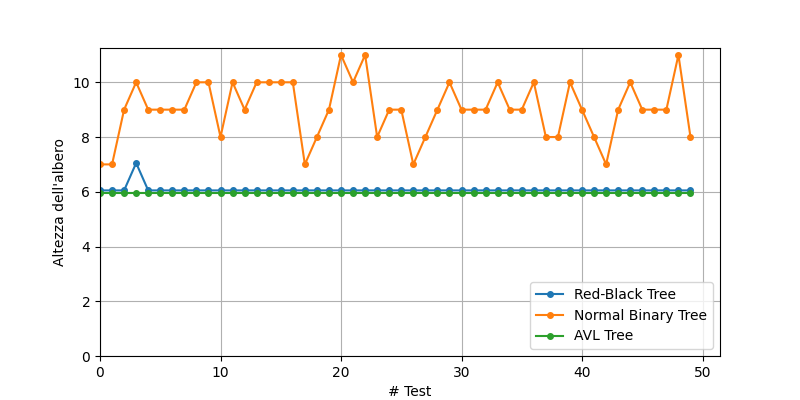
\includegraphics[width=\linewidth]{Altezza alberi}
            \caption{Altezza alberi con 31 nodi}
        \end{subfigure}
        \hfill
        \begin{subfigure}{0.49\textwidth}
            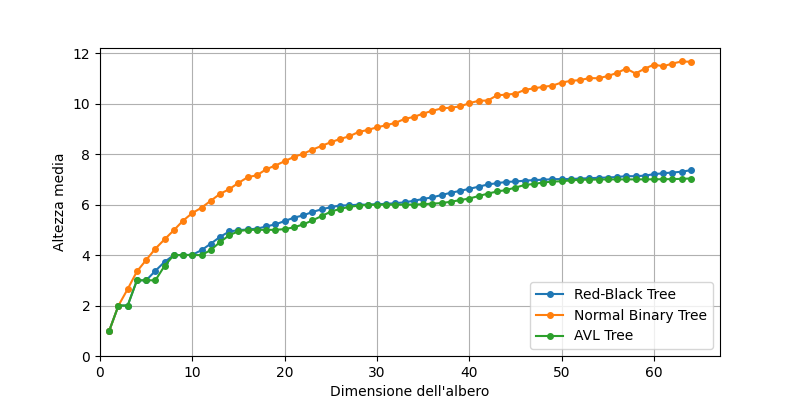
\includegraphics[width=\linewidth]{Altezza media}
            \caption{Altezza media con $n$ nodi}
        \end{subfigure}
        \caption{Altezza degli alberi}
    \end{figure}

    \subsubsection{Tempo medio di ricerca di un valore}
    L'ultimo test è quello relativo alla ricerca di un nodo nell'albero, di cui si vuole calcolare il tempo medio di
    esecuzione. Dato i risultati del test precedente, è ragionevole immaginare che, a parità di implementazione,
    la ricerca più veloce sarà quella che deve scorrere in media meno strati prima di giungere al nodo voluto,
    quindi gli alberi più performanti dovrebbero essere, in ordine, quello AVL, poi RN e infine l'albero binario
    normale.

    \begin{figure}[h]
        \centering
        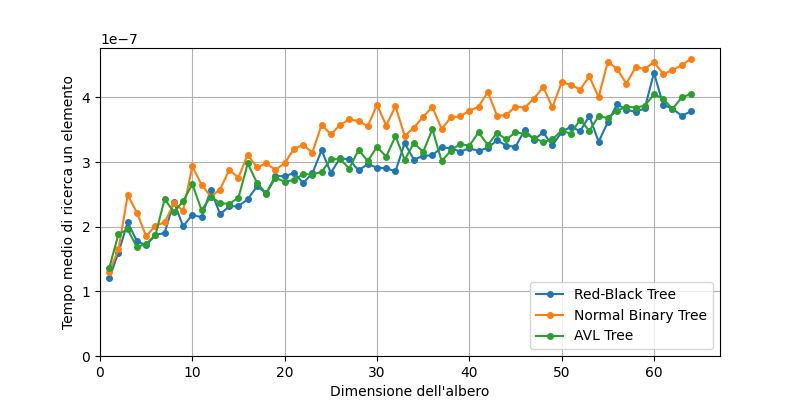
\includegraphics[width=1\textwidth]{Tempo medio di ricerca}
        \caption{Tempo medio di ricerca di un nodo}
        \label{fig:esempio}
    \end{figure}

    \subsubsection{Tempo medio di costruzione di un albero}
    In questo secondo test si prende in considerazione il tempo medio di inserimento/costruzione di un albero.
    Prendendone di nuovo uno per ogni tipo, vengono riempiti con una lista di valori interi da $1$ a $n$ e viene
    calcolato il tempo medio di inserimento del nodo e di costruzione totale dell'albero.

    \begin{figure}[htb!]
        \centering
        \begin{subfigure}{0.49\textwidth}
            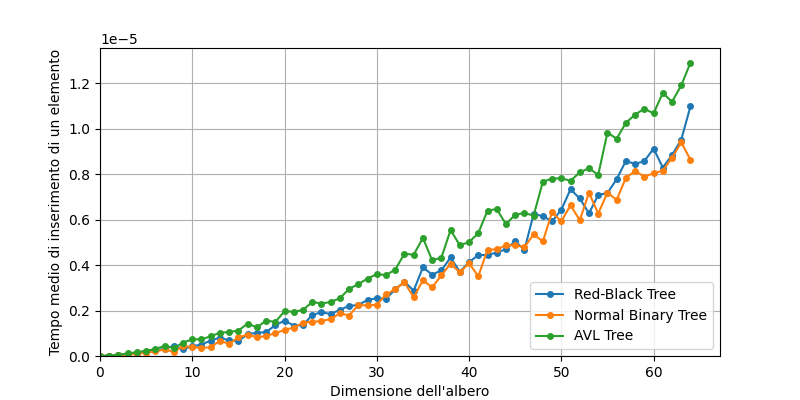
\includegraphics[width=\linewidth]{Tempo medio di inserimento}
            \caption{Tempo medio di inserimento di un nodo dato la dimensione dell'albero}
        \end{subfigure}
        \hfill
        \begin{subfigure}{0.49\textwidth}
            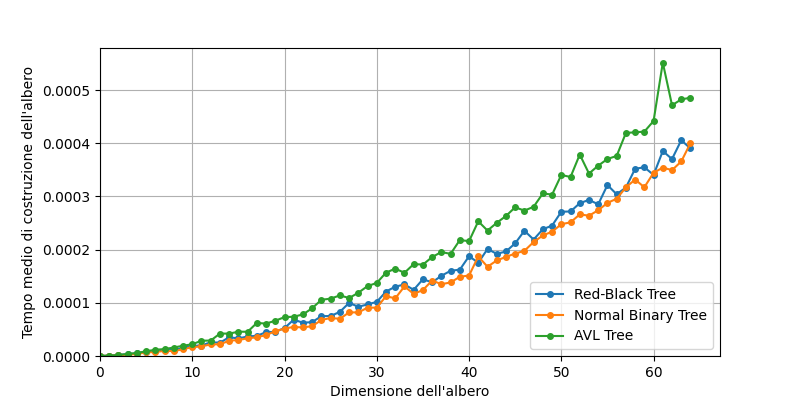
\includegraphics[width=\linewidth]{Tempo medio di costruzione}
            \caption{Tempo medio di costruzione dell'albero data la sua dimensione}
        \end{subfigure}
        \caption{Altezza degli alberi}
    \end{figure}

    \subsection{Analisi dei risultati sperimentali}
    Dal primo test risulta che, mentre l'albero binario normale ha un'altezza che oscilla tra tra 7 e 11, gli
    alberi rosso-nero e AVL hanno un'altezza quasi sempre pari a 6: questi risultati rispecchiano la natura
    auto-bilanciante degli ultimi due, che riescono a minimizzare la loro altezza grazie alle operazioni di rotazione
    successive all'inserimento.
    Inoltre si ha anche un primo indizio di quale dei due sia migliore: infatti dalla seconda figura si scopre che,
    mentre l'albero binario normale segue un andamento logaritmico molto "fluido", gli altri due sembrano procedere a
    scalini sempre più larghi, con l'altezza media dell'albero AVL sempre leggermente inferiore rispetto a quella
    dell'albero rosso-nero.
    \
    In particolare questi scalini si posizionano circa a 2, 4, 8, 14, 28, 48 nodi, con altezze relative di 2, 3, 4, 5, 6
    , 7: questa progressione conferma il teorema secondo cui un albero completo di altezza $n$ ha esattamente $2^n-1$
    nodi, infatti le altezze medie elencate approssimano le potenze di due con un difetto sempre più grande.
    Maggiore il numero di nodi e livelli, minore è la precisione nell'inserirne uno nuovo mantenendo a 1 la
    differenza tra altezza minima e massima.
    \vspace{\baselineskip}

    Il secondo test conferma esattamente quanto previsto, nonostante un po' di "rumore" nei risultati.
    \vspace{\baselineskip}

    Dai grafici ottenuti dall'ultimo test si riscontra che i due grafici hanno andamento simile ma su scale diverse, in
    quanto la costruzione non è altro che l'esecuzione di molti inserimenti in sequenza.

    In questo caso però, vediamo che le performance degli alberi sono invertite: per l'altezza media gli alberi
    che riuscivano a minimizzarla più efficacemente erano l'albero AVL e poi RN, in questo caso l'albero binario
    normale riesce a minimizzare il tempo di inserimento/costruzione, nonostante l'altezza media maggiore e la
    conseguente necessità, in media, di scendere più in profondità dell'albero per trovare la collocazione del nodo.

    Questo è causa dell'implementazione della funzione di inserimento, che mentre per l'albero binario normale
    preveda il semplice scorrimento dalla radice alla foglia, negli altri due casi necessita di un'ulteriore
    passaggio, rappresentato dalla funzione di fixup, che ristabilisca il bilanciamento dell'albero: questa sequenza
    di rotazioni e operazioni aggiuntive effettuate sui nodi e i loro attributi appesantisce l'inserimento, che ne
    risulta rallentato.

    \par\noindent\rule{\textwidth}{0.2pt}
    \section{Conclusioni}
    In conclusione, si può affermare che gli alberi rosso-nero e AVL sono più ottimizzati quando si devono eseguire
    ricerche e interrogazioni frequenti nella struttura dati, ma a causa della loro "costosa" operazione di
    inserimento, non sono la scelta migliore quando si vuole minimizzare il tempo di inserimento di nuovi dati.

    Al contrario, l'albero di ricerca binario è molto veloce nelle operazioni di inserimento (e cancellazione), ma
    non dà origine ad alberi bilanciati e ad una struttura dati ottimizzata.

    \par\noindent\rule{\textwidth}{0.2pt}
\end{document}
